%!TEX program = xelatex
\documentclass[cn,hazy,pku,12pt,normal,math=newtx,cite=super]{elegantnote}
\title{液体饱和蒸气压的测定}

\author{刘松瑞 \quad 2100011819 \\ 组号:24 \quad 组内编号:5}
\institute{化学与分子工程学院}

\expdate{\zhdate{2023/11/16}}
\temperature{18.3 \si{^{\circ}C}}
\pressure{102.05 \si{kPa}}

\usepackage{gensymb}
\usepackage{array}
\usepackage{subfigure}
\usepackage[fontset=windows]{ctex}
\usepackage{graphicx}
\usepackage{float}
\usepackage{caption}
\usepackage{multirow}
%\usepackage{subfig}
%\usepackage{float}
\begin{document}

\maketitle

\keywords{饱和蒸气压\quad摩尔气化焓\quad摩尔气化熵\quad褚鲁统规则}

\abstracts{
    本实验在不同温度下,采用静态法测定四氯化碳的饱和蒸气压,
计算得到四氯化碳的正常沸点为 
$(76.5 \pm 0.9)$ °C
,摩尔气化焓为 $ (31.43 \pm 0.07) \ {\rm kJ/mol}$
,摩尔气化熵为 $ (89.9 \pm 0.3)\ {\rm J/(mol\cdot K)}$;
然后采用动态法测定水的饱和蒸气压,
水的正常沸点为 $(99 \pm 2)$ °C
,摩尔气化焓为 $ (41.3 \pm 0.2) \ {\rm kJ/mol}$
,摩尔气化熵为 $ (111.0 \pm 0.8)\ {\rm J/(mol\cdot K)}$
。最后探究了温度计插入深度对动态法测量结果的影响,若插入过深会对测得的沸点温度造成显著误
差,因此应当将温度计置于液面处。
}

\newpage


\section{引言}

\subsection{实验目的与原理}

实验目的与原理详见预习报告图~\ref{1}。 \cite{pcl2002}

\begin{figure}[htbp]
    \centering
    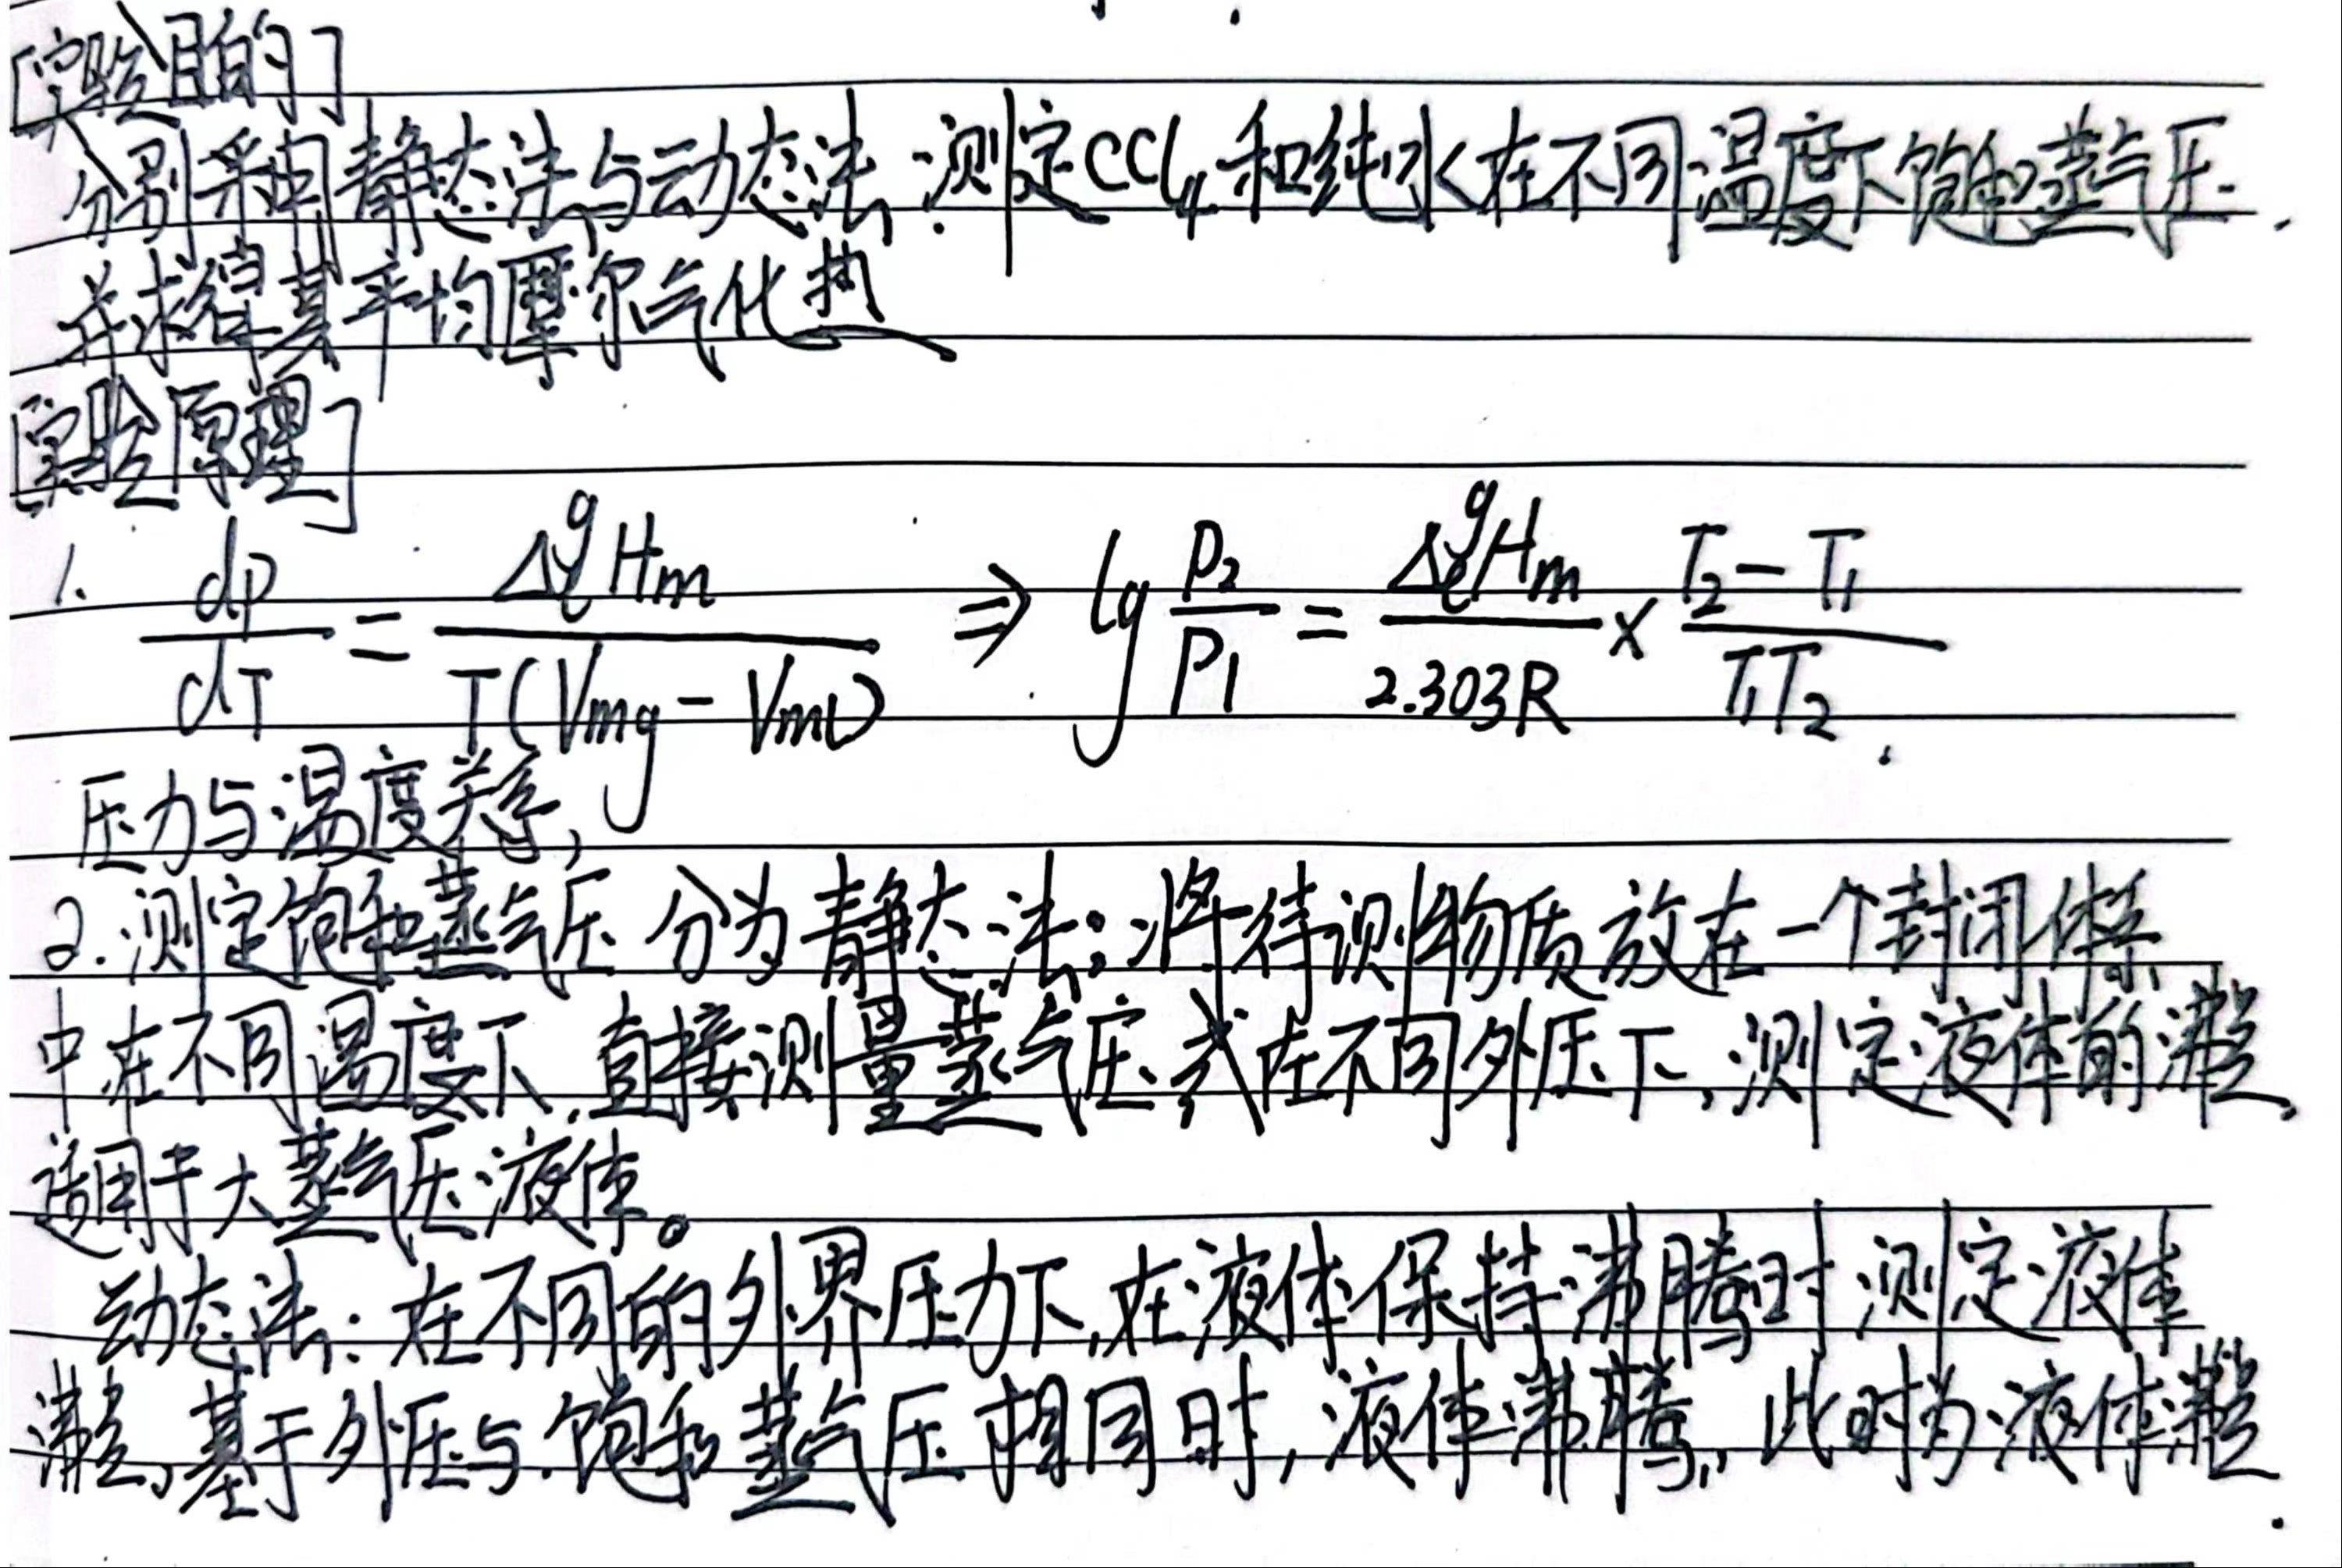
\includegraphics[width = .70\textwidth]{image/yxbg_1.jpg}
    \caption{实验的目的与原理}\label{1}
\end{figure}

\subsection{实验方法}

使用静态法与动态法测定 $\rm CCl_4$ 与 $\rm H_2O$ 的饱和蒸气压,得到工作曲线,并计算
 $\Delta^l_g H_m$。

\section{实验部分}

\subsection{实验步骤}
\subsubsection{静态法实验步骤}

\begin{enumerate}
    \item 向平衡管中加入适量四氯化碳,组装好实验装置,打开冷凝水,打开真空泵,打开真空泵连接储气罐的活塞,对体系减压约 50 kPa
    \item 关闭阀门,记录关闭阀门三分钟前后压力值变化为 0.01 kPa,说明装置气密性良好。
    \item 使体系与大气相通,将平衡管水浴加热至水浴温度达 80 $\rm \degree C$ 左右,
    保持加热数分钟,排除平衡管中空气与蒸气。
    \item 停止加热,不断搅拌。温度下降至两管液面达到同一水平的瞬间,
    立即记下此时的温度和压力,得到对应压力下的沸点。重复测定三次。
    \item 关闭通大气的活塞。打开通水泵的活塞减
    压约 5 kPa,冷却并不断搅拌。记录两管液面达到同一水平的瞬间的温度和压力。
    继续实验,每次减压 5 kPa,直到内外相差 50 kPa 时停止实验,此时再读一次大气压力。
    
\end{enumerate}

\subsubsection{动态法实验步骤}

\begin{enumerate}
    \item 组装测量系统并检查气密性:将两口圆底烧瓶加入约 200 mL 二次水,放入一个磁力搅拌子,
    适当搅拌防止暴沸。
    \item 减压至 50 kPa,记录关闭阀门三分钟前后压力值变化为 0.00 kPa,说明装置气密性良好。
    \item 调节外压,测量不同外压下的沸点,当烧瓶中水沸腾且温度不再上升时,记下温度压力数值,停止加热。
    \item 开启缓冲罐通大气的活塞,至压力值升高 5 kPa 左右,关闭活塞,重新加热。
    \item 最后一次使系统与大气完全相通,继续加热,记下沸腾时的温度。
\end{enumerate}

\subsection{仪器与药品}

\begin{enumerate} %有序列表
    \item 试剂 \\   四氯化碳,二次去离子水,1000 mL 烧杯,250 mL 两口圆底烧瓶。
    \item 仪器 \\   数字式温度-压力测定仪 (WXI-04 型),电加热器,循环水真空泵,带电热套的磁力
    搅拌装置,冷凝水循环系统,真空缓冲罐,直形冷凝管,搅拌磁子,真空脂。
\end{enumerate}

\section{实验现象与数据处理}
\subsection{静态法测四氯化碳的饱和蒸气压}
\subsubsection{常压下四氯化碳的沸点}

排气后,测量常压下四氯化碳的沸点,如表 \ref{01} 所示,由此可知:
$$
\bar{T} = 101.92 {\rm kPa} \quad \bar{p}  = 76.68 {\rm \degree C}
$$

\begin{table}[h]
    \centering
    \caption{常压下四氯化碳的沸点}
    \label{01}
    \begin{tabular}{ccc}
    \hline
      & T/$\rm \degree C$ & p/kPa  \\ \hline
    1 & 76.64         & 101.93 \\
    2 & 76.67         & 101.93 \\
    3 & 76.72         & 101.89 \\ \hline
    \end{tabular}
\end{table}


\subsubsection{不同气压下四氯化碳的饱和蒸气压}

测量不同气压下四氯化碳的沸点如表 \ref{02} ,对数据处理并线性回归得到图 \ref{2},
可以得到 $\ln(\frac{p}{p^o}) - \frac{1}{T}$ 线性关系为
$$
\ln(\frac{p}{p^o}) = (10.81 \pm 0.02) + (-3780 \pm 8) * \frac{1}{T} \quad R^2=0.99996
$$

\begin{table}[h]
    \centering
    \caption{不同气压下四氯化碳的沸点}
    \label{02}
    \begin{tabular}{ccccc}
    \hline
    p/kPa  & T/$\degree C$ & $\ln(p/p^o)$ & T/K    & $T^{-1}/K^{-1}$ \\ \hline
    101.92 & 76.68         & 0.0059       & 349.83 & 0.002859        \\
    91.97  & 73.41         & -0.0969      & 346.56 & 0.002886        \\
    82.54  & 69.91         & -0.2051      & 343.06 & 0.002915        \\
    78.12  & 68.21         & -0.2601      & 341.36 & 0.002929        \\
    73.31  & 66.24         & -0.3236      & 339.39 & 0.002946        \\
    68.26  & 64.11         & -0.3950      & 337.26 & 0.002965        \\
    62.76  & 61.61         & -0.4790      & 334.76 & 0.002987        \\
    57.40  & 59.02         & -0.5683      & 332.17 & 0.003011        \\
    50.14  & 55.14         & -0.7035      & 328.29 & 0.003046        \\ \hline
    \end{tabular}
\end{table}

数据测定结束后,测定大气压为 101.80 kPa,室温为 20.4 °C。

\begin{figure}[htbp]
    \centering
    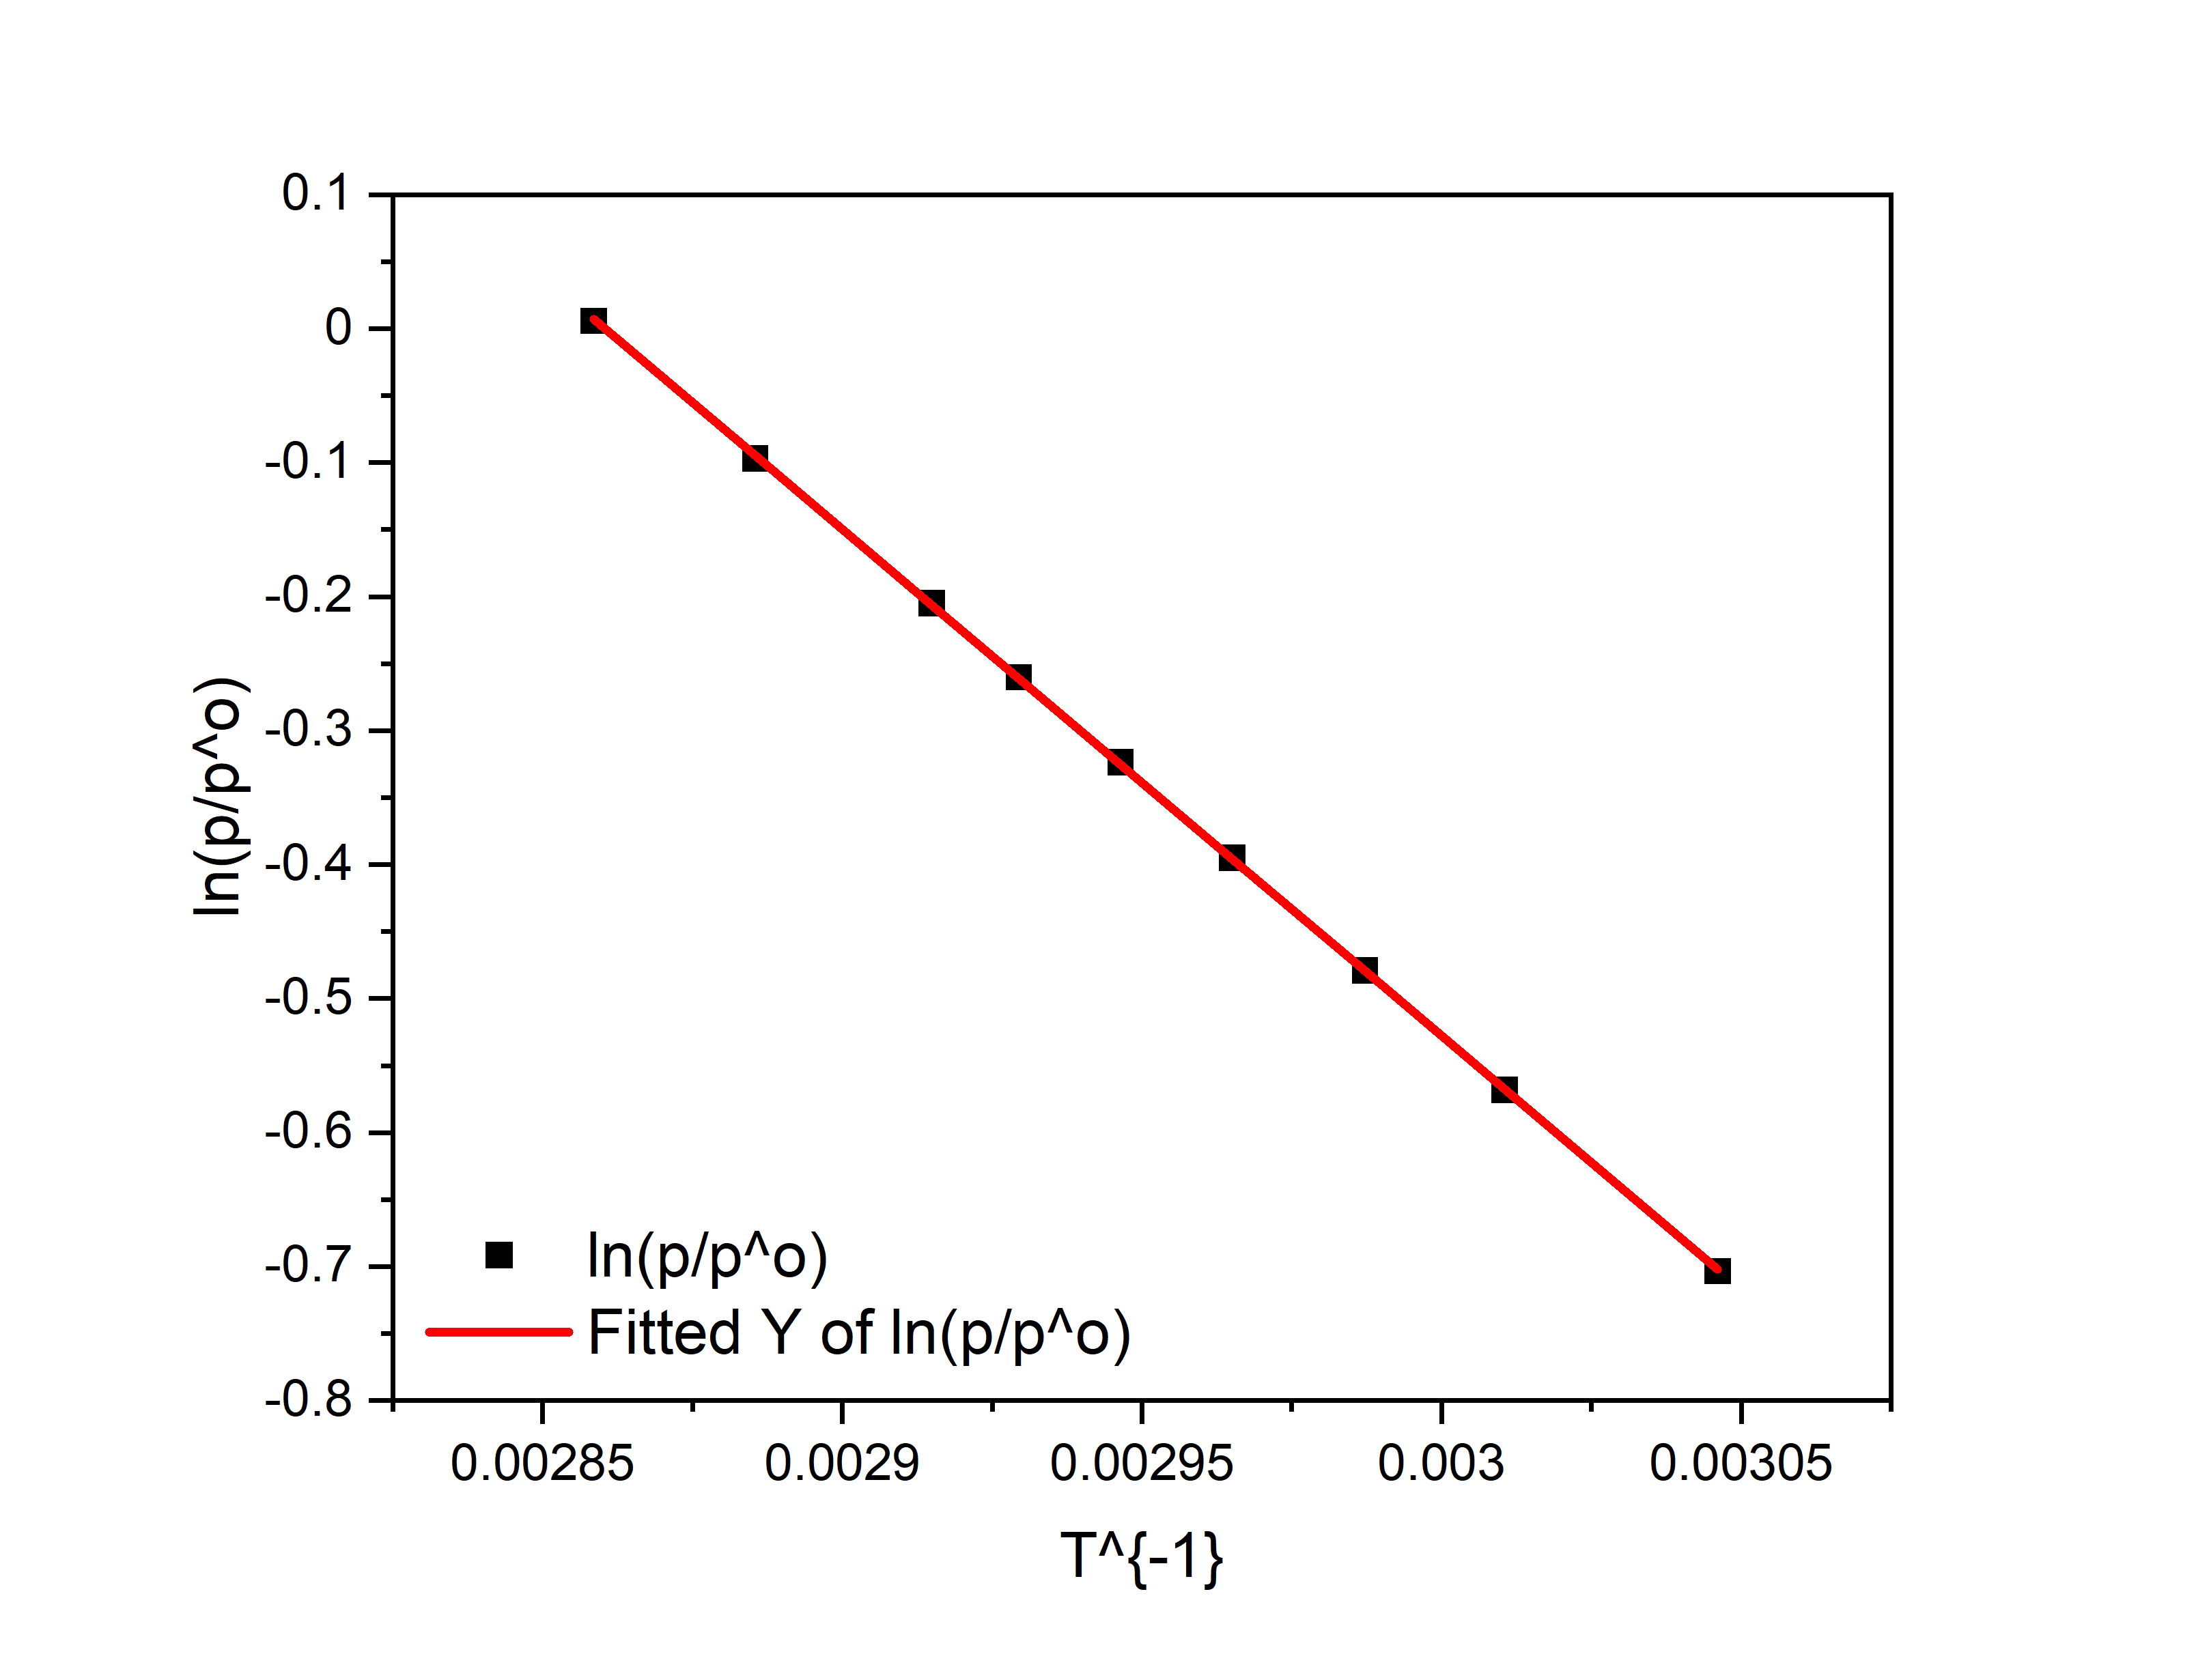
\includegraphics[width = .70\textwidth]{image/Graph4.png}
    \caption{四氯化碳的$\ln(\frac{p}{p^o}) - \frac{1}{T}$图}\label{2}
\end{figure}

计算在标准压力下,四氯化碳沸点为
$$
T_b = \frac{A}{\ln(\frac{p}{p^o})-B} = 349.7\ K
$$
$$
\sigma_{T_b} = T_b\sqrt{(\frac{\sigma_A}{A})^2+(\frac{\sigma_B}{\ln(\frac{p}{p^o})-B})^2} = 0.9\ K
$$

有 $T_b = 349.7 \pm 0.9\ K$,即 $76.5 \pm 0.9$ °C

由于 Clapeyron-Clausius 方程可知
$$
\ln(\frac{p}{p^o}) = \frac{\Delta^l_g H_m}{RT} + B
$$

可得
$$
\Delta^l_g H_m = - A \cdot R = (3.143 \times 10^4 \pm 7 \times 10^1) \ {\rm J/mol} = (31.43 \pm 0.07) \ {\rm kJ/mol}
$$

因此
$$
\Delta^l_g S_m = \frac{\Delta^l_g H_m}{T_b} = 89.9\ {\rm J/(mol \cdot K)}
$$
$$
\sigma_{\Delta^l_g S_m} = \Delta^l_g S_m\sqrt{(\frac{\sigma_{\Delta^l_g H_m}}{\Delta^l_g H_m})^2+(\frac{\sigma_{T_b}}{T_b})^2} = 0.3\ {\rm J/(mol \cdot K)}
$$

有 $\Delta^l_g S_m = 89.9 \pm 0.3\  {\rm J/(mol\cdot K)}$,这与褚鲁统规则基本一致。

\subsection{动态法测水的饱和蒸气压}

测量不同气压下水的沸点如表 \ref{03} ,对数据处理并线性回归得到图 \ref{3},
可以得到 $\ln(\frac{p}{p^o}) - \frac{1}{T}$ 线性关系为
$$
\ln(\frac{p}{p^o}) = (13.36 \pm 0.06) + (-4.97 \times 10^3 \pm 2 \times 10^1) * \frac{1}{T} \quad R^2=0.9992
$$

\begin{table}[h]
    \centering
    \caption{不同气压下水的沸点}
    \label{03}
    \begin{tabular}{ccccc}
    \hline
    p/kPa  & T/$\degree C$ & $\ln(p/p^o)$ & T/K    & $T^{-1}/K^{-1}$ \\ \hline
    51.00  & 80.20         & -0.6865      & 353.35 & 0.002830        \\
    56.75  & 83.07         & -0.5797      & 356.22 & 0.002807        \\
    64.28  & 86.34         & -0.4551      & 359.49 & 0.002782        \\
    77.04  & 90.93         & -0.2740      & 364.08 & 0.002747        \\
    82.71  & 92.95         & -0.2030      & 366.10 & 0.002731        \\
    84.17  & 93.46         & -0.1855      & 366.61 & 0.002728        \\
    91.22  & 95.49         & -0.1051      & 368.64 & 0.002713        \\
    95.59  & 96.81         & -0.0583      & 369.96 & 0.002703        \\
    101.80 & 98.59         & 0.0047       & 371.74 & 0.002690        \\ \hline
    \end{tabular}
\end{table}

数据测定结束后,测定大气压为 101.73 kPa,室温为 20.7 °C。

\begin{figure}[htbp]
    \centering
    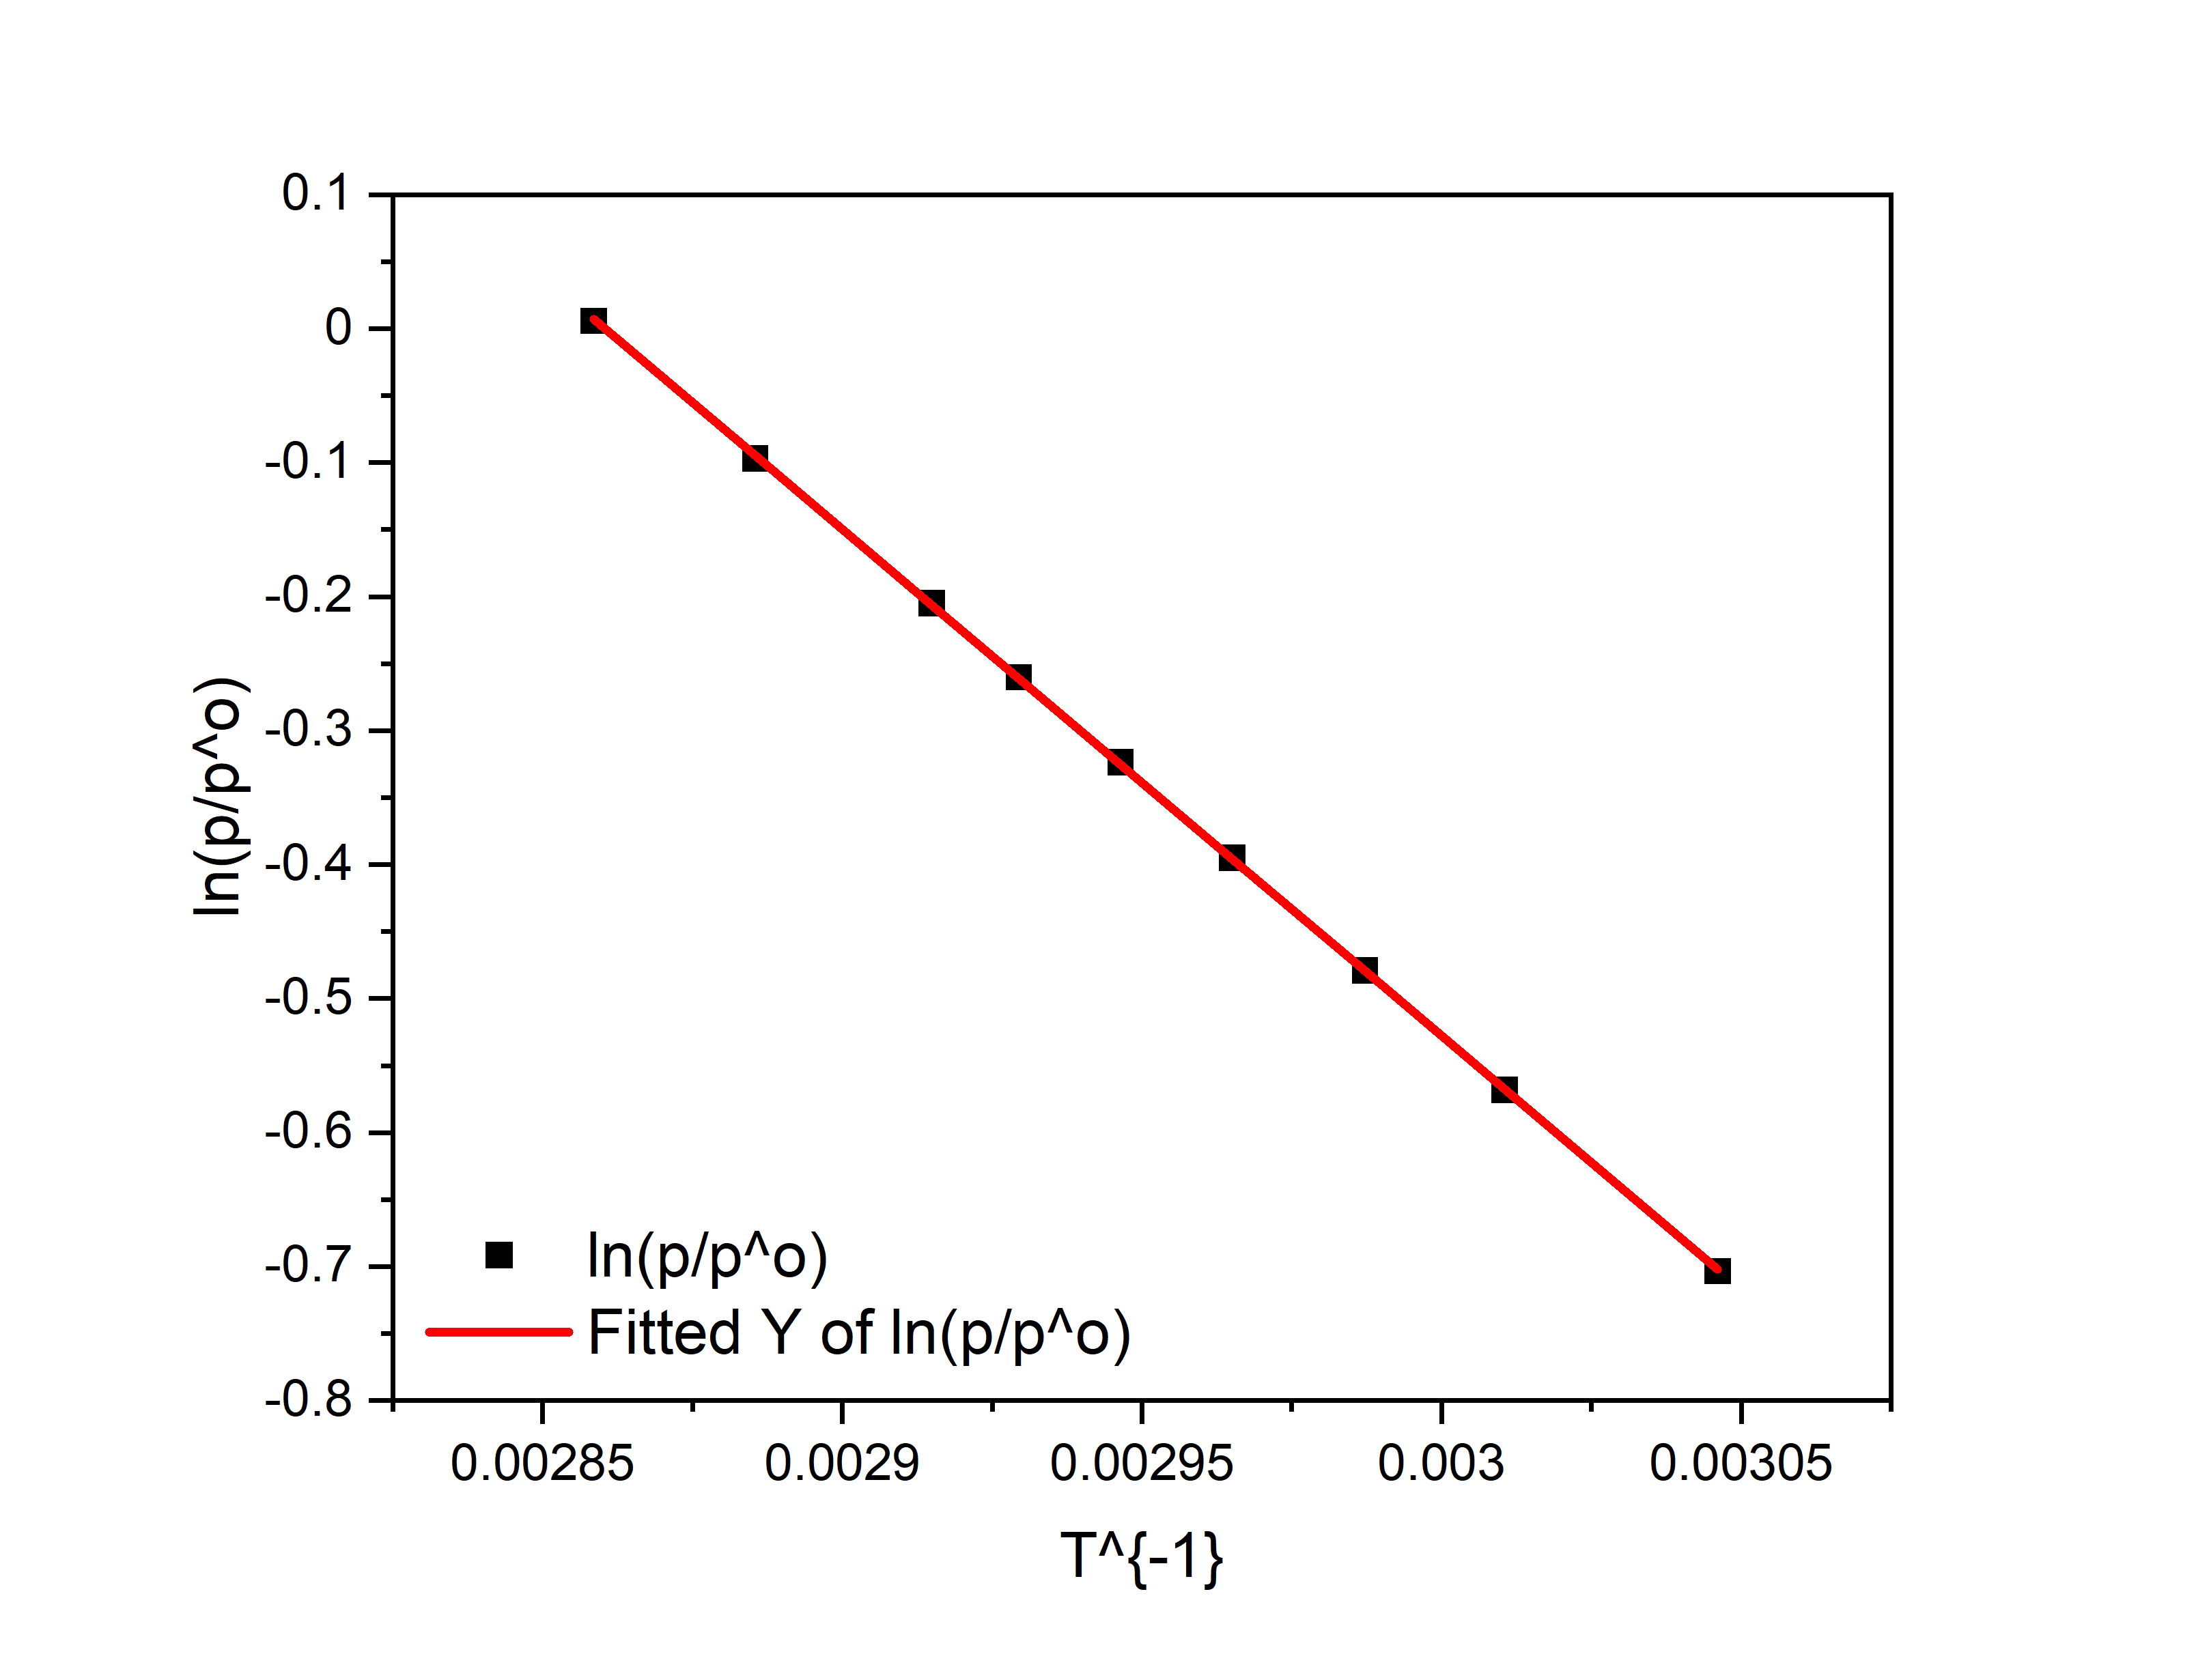
\includegraphics[width = .70\textwidth]{image/Graph4.png}
    \caption{水的$\ln(\frac{p}{p^o}) - \frac{1}{T}$图}\label{3}
\end{figure}


计算在标准压力下,水的沸点为
$$
T_b = \frac{A}{\ln(\frac{p}{p^o})-B} = 372\ K
$$
$$
\sigma_{T_b} = T_b\sqrt{(\frac{\sigma_A}{A})^2+(\frac{\sigma_B}{\ln(\frac{p}{p^o})-B})^2} = 2\ K
$$

有 $T_b = 372 \pm 2\ K$,即 $(99 \pm 2)$ °C。

摩尔气化焓为
$$
\Delta^l_g H_m = A \cdot R = (4.13 \times 10^4 \pm 2 \times 10^2) \ {\rm J/mol} = (41.3 \pm 0.2) \ {\rm kJ/mol}
$$

因此摩尔气化熵为
$$
\Delta^l_g S_m = \frac{\Delta^l_g H_m}{T_b} = 111.0\ {\rm J/(mol \cdot K)}
$$
$$
\sigma_{\Delta^l_g S_m} = \Delta^l_g S_m\sqrt{(\frac{\sigma_{\Delta^l_g H_m}}{\Delta^l_g H_m})^2+(\frac{\sigma_{T_b}}{T_b})^2} = 0.8\ {\rm J/(mol \cdot K)}
$$

有 $\Delta^l_g S_m = 111.0 \pm 0.8\ {\rm J/(mol\cdot K)}$,这与褚鲁统规则相差较大。


\section{实验结果与讨论}

\subsection{讨论}
\subsubsection{与标准值的比较与误差分析}

查阅文献\cite{Weast1988CRC}可知,对四氯化碳有
$$
T = 349.85\ {\rm K} \quad \Delta^l_g H_m = 29.82\ {\rm J/mol} \quad \Delta^l_g S_m = 85.24\ {\rm J/(mol\cdot K)}
$$

可以以此计算测量误差
$$
E_r(T) = \frac{349.7-349.85}{349.85} = 0.04 \%
$$
$$
E_r(\Delta^l_g H_m) = \frac{31.43-29.82}{29.82} = 5.4 \% 
$$
$$
E_r(\Delta^l_g S_m) = \frac{89.9 -85.24}{85.24} = 5.5 \% 
$$

对水有
$$
T = 373.15\ {\rm K} \quad \Delta^l_g H_m = 40.65\ {\rm kJ/mol} \quad \Delta^l_g S_m = 108.95\ {\rm J/(mol\cdot K)}
$$
$$
E_r(T) = \frac{373 - 373.15}{373.15} = -0.3 \%
$$
$$
E_r(\Delta^l_g H_m) = \frac{41.3-40.65}{40.65} = 1.6 \% 
$$
$$
E_r(\Delta^l_g S_m) = \frac{111.0-108.95}{108.95} = 1.9 \% 
$$

由于两种液体在升温过程中摩尔气化焓和摩尔气化熵会发生变化,而我们使用的 Clapeyron - Clausius 方程
忽略了这一点,近似认为摩尔气化焓和摩尔气化熵不变,因此在于沸点时的真实值进行比较会有显著的误差。
此外,在计算时近似认为气体为理想气体也会带来一定误差。

对于四氯化碳这样的非极性分子,分子间相互作用小,因此可以较好地符合褚鲁统规则。水分子间有氢键相互作用
且为极性分子,与理想液体的偏离较大。因此水的摩尔气化熵显著偏离常数,不符合褚鲁统规则。

\subsubsection{温度计插入深度对动态法测量的影响}

对于正常情况,温度计应当放置在液面处,但是液体沸腾时存在一定的温度梯度,可能会造成一定的误差。
因此,笔者探究温度计放置位置对测量结果的影响。在实验中,笔者将温度计伸入液面,进行动态法测量。
同样地,得到不同气压下水的沸点如表 \ref{04} ,对数据处理并线性回归得到图 \ref{4},
可以得到 $\ln(\frac{p}{p^o}) - \frac{1}{T}$ 线性关系为
$$
\ln(\frac{p}{p^o}) = (13.37 \pm 0.05) + (-5.00 \times 10^3 \pm 2 \times 10^1) * \frac{1}{T} \quad R^2=0.9999
$$

\begin{table}[h]
    \centering
    \caption{不同气压下水的沸点}
    \label{04}
    \begin{tabular}{ccccc}
    \hline
    p/kPa  & T/$\degree C$ & $\ln(p/p^o)$ & T/K    & $T^{-1}/K^{-1}$ \\ \hline
    50.55  & 82.03         & -0.6954      & 355.18 & 0.002815        \\
    54.75  & 84.22         & -0.6156      & 357.37 & 0.002798        \\
    59.60  & 86.39         & -0.5307      & 359.54 & 0.002781        \\
    65.18  & 88.77         & -0.4412      & 361.92 & 0.002763        \\
    69.66  & 90.49         & -0.3747      & 363.64 & 0.002750        \\
    74.73  & 92.40         & -0.3045      & 365.55 & 0.002736        \\
    79.28  & 93.94         & -0.2453      & 367.09 & 0.002724        \\
    84.80  & 95.74         & -0.1780      & 368.89 & 0.002711        \\
    89.46  & 97.21         & -0.1245      & 370.36 & 0.002700        \\
    94.42  & 98.67         & -0.0706      & 371.82 & 0.002689        \\
    101.73 & 100.64        & 0.0040       & 373.79 & 0.002675        \\ \hline
    \end{tabular}
\end{table}

\begin{figure}[htbp]
    \centering
    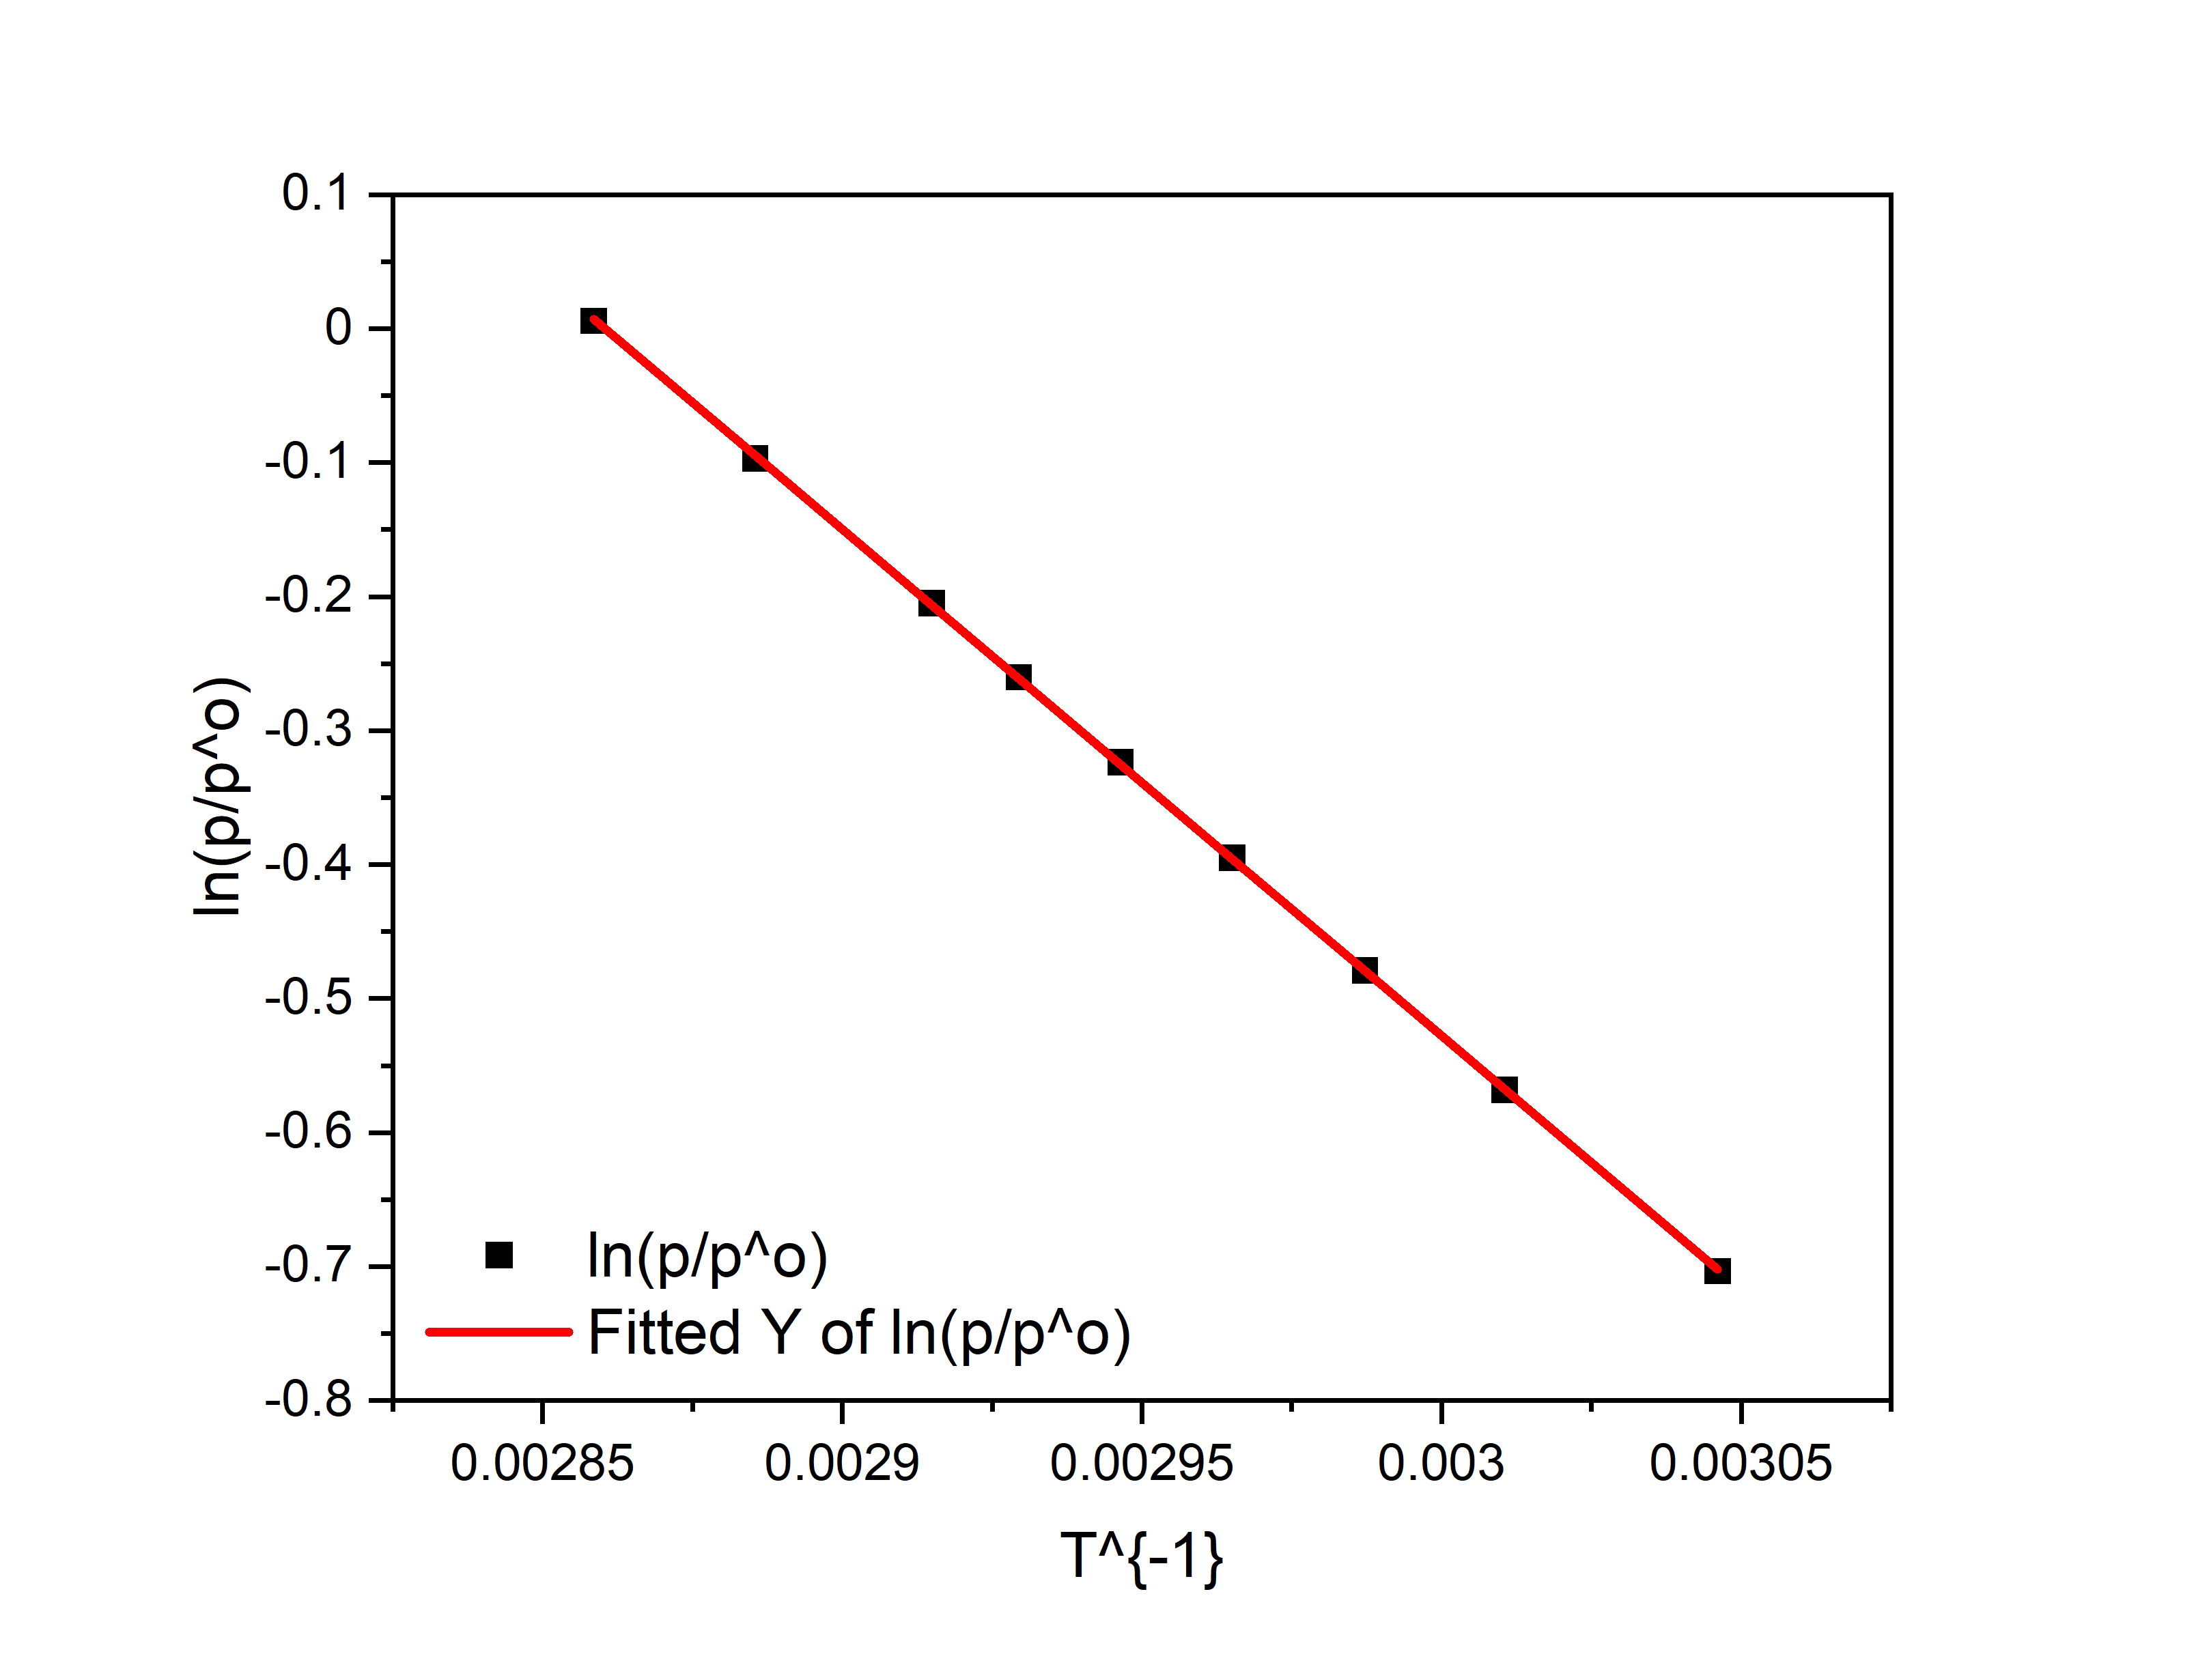
\includegraphics[width = .70\textwidth]{image/Graph4.png}
    \caption{水的$\ln(\frac{p}{p^o}) - \frac{1}{T}$图}\label{4}
\end{figure}


计算在标准压力下,水的沸点为
$$
T_b = \frac{A}{\ln(\frac{p}{p^o})-B} = 374\ K
$$
$$
\sigma_{T_b} = T_b\sqrt{(\frac{\sigma_A}{A})^2+(\frac{\sigma_B}{\ln(\frac{p}{p^o})-B})^2} = 2\ K
$$

有 $T_b = 374 \pm 2\ K$,即 $(101 \pm 2)$ °C。

反应的摩尔气化焓为
$$
\Delta^l_g H_m = A \cdot R = (4.13 \times 10^4 \pm 2 \times 10^2) \ {\rm J/mol} = (41.3 \pm 0.2) \ {\rm kJ/mol}
$$

因此摩尔气化熵为
$$
\Delta^l_g S_m = \frac{\Delta^l_g H_m}{T_b} = 110.4\ {\rm J/(mol \cdot K)}
$$
$$
\sigma_{\Delta^l_g S_m} = \Delta^l_g S_m\sqrt{(\frac{\sigma_{\Delta^l_g H_m}}{\Delta^l_g H_m})^2+(\frac{\sigma_{T_b}}{T_b})^2} = 0.7\ {\rm J/(mol \cdot K)}
$$

得到 $\Delta^l_g S_m = 110.4 \pm 0.7\ {\rm J/(mol\cdot K)}$。

与标准沸点相比较
$$
E_r(T) = \frac{374 - 373.15}{373.15} = 0.2 \%
$$

对比两次试验结果,可以发现,将温度计插入较深会导致测得的沸点升高,因为此时温度计更接近热源,
液体发生过热现象。而我们得到的摩尔气化熵与摩尔气化焓与之前的差异并不明显,仅摩尔气化熵略微增加。
综上,我们在进行实验时为得到准确的蒸气温度,仍然应当将温度计置于液面处,若插入过深会对测得的沸点温度造成显著误差。

\subsection{结论}

本实验在不同温度下,采用静态法测定四氯化碳的饱和蒸气压,
计算得到四氯化碳的正常沸点为
$(76.5 \pm 0.9)$ °C
,摩尔气化焓 $\Delta^l_g H_m = (31.43 \pm 0.07) \ {\rm kJ/mol}$
,摩尔气化熵 $\Delta^l_g S_m = (89.9 \pm 0.3)\ {\rm J/(mol\cdot K)}$;
然后采用动态法测定水的饱和蒸气压,
水的正常沸点为 $(99 \pm 2)$ °C
,摩尔气化焓 $\Delta^l_g H_m = (41.3 \pm 0.2) \ {\rm kJ/mol}$
,摩尔气化熵 $\Delta^l_g S_m = (111.0 \pm 0.8)\ {\rm J/(mol\cdot K)}$
。最后探究了温度计插入深度对动态法测量结果的影响,若插入过深会对测得的沸点温度造成显著误
差,因此应当将温度计置于液面处。


\nocite{*}
\bibliography{reference}
\end{document}
